\section{Các khái niệm về xác suất}
\subsection{Hàm mật độ xác suất (Probability density function)}
Với các phiên giao dịch có các thành phần như giá mở, giá đóng, số lượng đồng giao dịch,\dots, ta có thể coi như các biến ngẫu nhiên liên tục tương ứng. Khái niệm hàm mật độ xác suất trong văn cảnh trên được hiểu như một hàm gồm các tham số thể hiện được mật độ phân bố của các biến ngẫu nhiên.
\begin{figure}[hbt!]
	\center	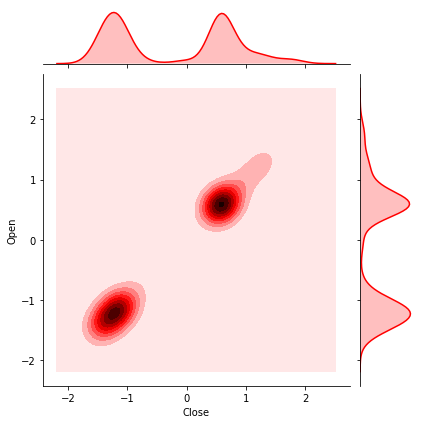
\includegraphics[width=0.8\textwidth]{probability/z_score_marginal_distribute_diff.png}
	\caption{Phân phối biên giá mở/đóng dữ liệu đã xử lý}
	\label{fig:z_score_marginal_distribution_diff}
\end{figure}
\FloatBarrier
Hình ~\ref{fig:z_score_marginal_distribution_diff} thể hiện mật độ của phân phối đồng thời giữa giá đóng và giá mở của các khối nến được biểu diễn dưới dạng $p_{data}(Open, Close)$.
\subsection{Hàm phân phối biên (Marginal distribution)}
Với dữ liệu liên tục như trên, hàm phân phối biên đối với giá mở được biểu diễn dưới dạng:
$p_{data}(Open) = \int_y p_{data}(Open, Close=y) dy = \int_y p_{data}(Open \given Close=y)p_{data}(Close=y)dy$ Một cách trực quan, hàm phân phối trên được biểu diễn bởi đường biên bên trái Hình ~\ref{fig:z_score_marginal_distribution_diff}

\subsection{Nhiễu trắng (White noise)}
Nhiễu trong dữ liệu như phần đề cập trong phần \ref{concept:finance:noise} có thể được giảm thiểu bằng cách tìm hàm phân phối của nhiễu bằng thống kê, nếu phân phối của nhiễu có dạng phân phối chuẩn với trung bình là 0, nhiễu này được gọi là nhiễu trắng Gauss (white Gaussian noise). Việc giảm thiểu nhiễu trong dữ liệu làm mô hình trở nên dễ tìm được mẫu đặc trưng (pattern) hơn.

\subsection{Biến ẩn (Latent variable)}
Biến ẩn được hiểu theo cách trừu tượng là biến không thể quan sát trực tiếp\cite[trang~264]{bishop} mà được suy luận từ biến quan sát được trong dữ liệu. Cụ thể hơn, với dữ liệu là giá của 100 ngày đầu một mô hình có khả năng tìm được quan hệ giữa giá ngày thứ 50 phụ thuộc nhiều vào giá ngày thứ 49 hơn so với ngày thứ 99, mô hình này được gọi là mô hình biến ẩn (latent variable model) với quan hệ được biểu diễn bằng phép toán có giá trị được lưu trong các biến ẩn.
\subsection{Mô hình đồ thị có hướng (Directed graphical model)}
Trong mô hình đồ thị có hướng hay mạng Bayes (Bayes network) việc suy diễn từ các trạng thái trước sang các trạng thái sau.
\begin{figure}[hbt!]
	\center	\includegraphics[width=0.6\textwidth]{Variational_inference/Bayes_inference.png}
	\caption{Mô hình mạng Bayes}
	\label{fig:Bayes_inference}
\end{figure}
Cụ thể với mô hình được được trực quan theo như Hình ~\ref{fig:Bayes_inference}, một giao dịch BTC/USD vào 6 giờ sáng ngày 31/7/2017 có giá mở là 2439.97\$, giá đóng là 2415.19\$, lượng giao dịch là 138.82 đồng BTC với xu hướng giao dịch tiếp theo có xác suất được kí hiệu là:
$P(Up \given Open =2727.26, Close=2740.01, Volume BTC = 385.41)$ với xác suất đồng thời của giao dịch và được tính:\\
$
P(Up,Open =2727.26, Close=2740.01, Volume BTC = 385.41)\\
 = P(Up| Pa(Up)) \cdot P(Up | P_1)
\cdot P(Open|Pa(Up)) \cdot P(Open|P_1)\cdot P(Close|Pa(Up))\\
\cdot P(Close|P_1) \cdot P(Volume BTC|Pa(Up)) \cdot P(Volume BTC|P_1)
$\\
Một cách tổng quát xác suất đồng thời của giao dịch và xu hướng tăng giảm về giá của giao dịch tiếp theo được biểu diễn dưới dạng:
$p_\theta(x_1, x_2, \dots, x_M) = \prod_{i=1}^{M}p_\theta(x_j, Pa(x_j))$ với $Pa(x_j)$ biến cha (parent variable) của $x_j$.
\subsection{Suy luận biến phân (Variational inference)}
Phương pháp suy luận biến phân được sử dụng trong mô hình đồ thị có hướng\cite{intro_variational} với các biến ẩn $z$ và các quan sát $x$ với mục tiêu ước lượng được phân bố của $x$ được xấp xỉ bằng phân phối $Q(Z)$: $P(X \given Z) \approx Q(Z)$ với $Q(Z)$ là phân phối tiên nghiệm đơn giản hơn $P(Z|X)$.

Sử dụng độ đo bất đồng Kullback–Leibler nhằm thể hiện sự khác nhau giữa phân phối $Q$ so với phân phối $P$: 


$\Dkl{Q}{P} \triangleq  \mathbb{E}_{Q(Z)} [\log \frac{Q(Z)}{P(Z \given X)}]$

Sử dụng luật Bayes:
$\Dkl{P}{Q} = \mathbb{E}_{Q(Z)} [\log \frac{Q(z)}{P(z , x)}  + \log P(x)]$\\
hay:\\
$\log(P(x)) = \Dkl{P}{Q} - \mathbb{E}_{Q(z)} [\log \frac{Q(z)}{P(z , x)}]
= \Dkl{P}{Q} + \mathcal{L}(Q)
$
